\documentclass[conference]{IEEEtran}
\IEEEoverridecommandlockouts
\usepackage{cite}
\usepackage{amsmath,amssymb,amsfonts}
\usepackage{algorithm}
\usepackage{algpseudocode}
\usepackage{graphicx}
\usepackage{booktabs}
\usepackage{textcomp}
\usepackage{xcolor}
\usepackage{url}
\usepackage{tikz}
\usetikzlibrary{arrows.meta,positioning,fit,backgrounds}

\begin{document}

\title{Learnova: Rebuilding Lecture Slide Decks into\\Visually Structured, Interactive Presentations}

\author{
\IEEEauthorblockN{Kawaljeet Singh Bharaj, Jeevesh Bharat Bodhani, Rishit Pankajkumar Lahoti, Swayam Devendra Panchal}
\IEEEauthorblockA{Department of Artificial Intelligence and Data Science\\
Dwarkadas J. Sanghvi College of Engineering, Mumbai, India\\
panchalswayam35@gmail.com}
}

\maketitle

\begin{abstract}
Most lecture slides that students receive are exported PowerPoint files or PDFs made of dense bullet lists, pictures of
equations and diagrams with no structure a program can use. Tools that generate presentations from a prompt do not help
much here: they start from scratch, paraphrase the teacher's content and cannot be checked against the source. We describe
Learnova, a system that takes an existing deck (PPTX, slide PDF, Word document or typed notes) and rebuilds it as an
editable PowerPoint file and an interactive web deck while keeping every point the teacher wrote. The system has four
parts: a page-by-page reader that recovers titles, bullet nesting, tables and figures from slide PDFs, including slides
that are only pictures; a rule-based Content Decision Engine that chooses a visual form for each slide (process, timeline,
comparison table, definition, chart and others) with a stated reason; a layout stage that measures text glyph by glyph so
that no word is ever broken across lines; and an illustration stage that draws a diagram for every topic slide, written by
a language model when an API key is available and drawn by offline rules when it is not. On three held-out gold sets
(101 slides) the decision engine picked an acceptable visual for 96.8--97.4\% of slides in under one millisecond per
slide. On six real course decks (36 to 216 pages) the rebuilt decks kept 98--100\% of numeric and named facts, and the
layout audit flagged at most 4\% of slides, none of them for broken words.
\end{abstract}

\begin{IEEEkeywords}
presentation generation, document layout analysis, educational technology, slide redesign, information visualisation,
large language models
\end{IEEEkeywords}

\section{Introduction}
A typical engineering course in our college is taught from slide decks that have been reused for years. When we collected
decks from our own semester---natural language processing, machine learning and image processing---we found the same
pattern in all of them: long bullet lists, equations pasted as screenshots, diagrams copied from textbooks, and many
slides with no title at all. Students read these decks before examinations, and they are not easy to read.

Recent tools such as Gamma~\cite{gamma}, Copilot in PowerPoint~\cite{copilotppt}, Gemini in Google
Slides~\cite{geminislides} and Canva Magic Design~\cite{canva} make attractive decks from a short prompt. They are
designed for creating new presentations rather than repairing old ones. When a lecture deck is pasted into them, the
content is rewritten, items of a list are silently dropped, and the result cannot be compared with the original. For
a study aid that is a serious problem: the student cannot tell which point went missing. Abstractive summarisers are known
to make exactly these errors~\cite{maynez2020,ji2023}.

Learnova takes the opposite position. The teacher's content is treated as fixed, and the system only changes how it is
shown. Our contributions are:
\begin{itemize}
\item a reader that turns a slide deck exported to PDF (and, through a PDF rendering, a PPTX file) back into structured
slides, including OCR for picture-only slides and recovery of wrapped titles and split words;
\item a deterministic Content Decision Engine that maps each slide to one of more than twenty visual families and returns
the data that visual needs together with a reason;
\item a glyph-measured text-fitting method and a layout audit that guarantee that words are never split across lines;
\item a per-slide illustration stage with two fallbacks: a diagram written as SVG by a language model under strict
validation, and an offline scene illustrator;
\item an evaluation on gold sets and on six real course decks, with all numbers reproducible from the repository.
\end{itemize}

\section{Related Work}
\textit{Document-to-slide generation.} PPSGen~\cite{hu2015} learned sentence importance to build slides from papers;
DOC2PPT~\cite{fu2022} and D2S~\cite{sun2021} generate slides from scientific documents with neural summarisation and
figure selection. These systems target papers, not existing decks, and they summarise rather than preserve content.

\textit{Commercial deck generators.} Gamma, Copilot, Gemini and Canva generate an outline first and then fill a template.
In our trials they produced good-looking slides but changed wording, merged list items and could not keep the original
figures of an uploaded lecture.

\textit{Automatic visual design.} Mackinlay's APT~\cite{mackinlay1986} chose graphical encodings from data
characteristics, and Draco~\cite{moritz2019} encodes visualisation design knowledge as constraints. Our decision engine
follows the same idea---explicit, inspectable rules---but applies it to sentences rather than data tables.

\textit{Slide design guidance.} Assertion--evidence slides, which use a sentence headline supported by a visual, improve
comprehension over bullet lists~\cite{alley2006,garner2013}. Mayer's multimedia principles~\cite{mayer2009} and cognitive
load theory~\cite{sweller1988} motivate keeping related text and pictures together and limiting the number of new items
on a slide. Tufte's critique of bullet outlines~\cite{tufte2003} is another source of the problem we address.

\textit{Line breaking.} Knuth and Plass~\cite{knuth1981} treated paragraph layout as an optimisation over break points.
We need a much simpler guarantee---no word wider than its box---but in many small boxes at once.

\section{System Overview}
Fig.~\ref{fig:arch} shows the pipeline. An upload is converted into a Markdown intermediate representation together with
per-slide metadata (figures, page previews, OCR text, colour palette of the source). The planner splits overloaded slides
and merges very short ones; the enrichment stage adds an agenda, checkpoint quizzes, key terms and a glossary; the
decision engine picks a visual for each slide; the illustration and lab stages prepare pictures and interactive pages; and
two builders write the PowerPoint file (python-pptx, native editable shapes) and the web deck (Reveal.js~\cite{revealjs}).
A FastAPI service runs jobs in the background and a React front end shows progress, previews and exports.

\begin{figure}[t]
\centering
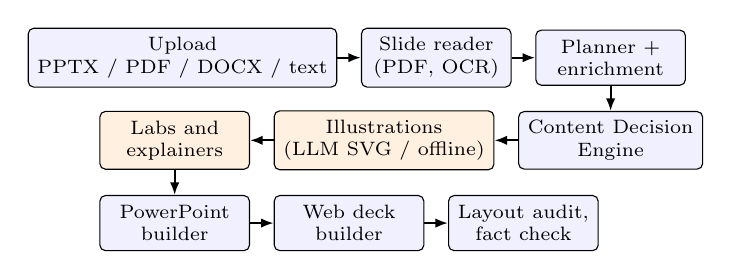
\begin{tikzpicture}[node distance=3.2mm and 3mm, font=\scriptsize,
  box/.style={draw, rounded corners=2pt, fill=blue!6, align=center, minimum width=19mm, minimum height=7mm},
  opt/.style={draw, rounded corners=2pt, fill=orange!12, align=center, minimum width=19mm, minimum height=7mm},
  arr/.style={-{Latex[length=1.6mm]}, thick}]
\node[box] (in) {Upload\\PPTX / PDF / DOCX / text};
\node[box, right=of in] (read) {Slide reader\\(PDF, OCR)};
\node[box, right=of read] (plan) {Planner +\\enrichment};
\node[box, below=of plan] (dec) {Content Decision\\Engine};
\node[opt, left=of dec] (ill) {Illustrations\\(LLM SVG / offline)};
\node[opt, left=of ill] (lab) {Labs and\\explainers};
\node[box, below=of lab] (ppt) {PowerPoint\\builder};
\node[box, right=of ppt] (web) {Web deck\\builder};
\node[box, right=of web] (aud) {Layout audit,\\fact check};
\draw[arr] (in) -- (read); \draw[arr] (read) -- (plan); \draw[arr] (plan) -- (dec);
\draw[arr] (dec) -- (ill); \draw[arr] (ill) -- (lab);
\draw[arr] (lab) -- (ppt); \draw[arr] (ppt) -- (web); \draw[arr] (web) -- (aud);
\end{tikzpicture}
\caption{Learnova pipeline. Orange stages use a language model when a key is set and fall back to offline rules otherwise.}
\label{fig:arch}
\end{figure}

\section{Reading Slide Decks}
\label{sec:reader}
A slide PDF already contains one slide per page, but its structure is implicit. The reader works on text lines from
PyMuPDF, each with a bounding box $(x_0,y_0,x_1,y_1)$, a font size $s$ and a font name.

\textit{Furniture removal.} A line in the top 12\% or bottom 14\% of a page is treated as page furniture (course name,
author, slide number) when the same normalised text appears in that band on at least
\begin{equation}
m = \max\bigl(3,\ \lfloor 0.3\,n \rfloor\bigr)
\end{equation}
of the $n$ pages. Page counters of the form ``$k/n$'' and the chrome of decks exported by slide tools are removed as well.
Repeated pictures are handled in the same way, but we count only images actually drawn on a page: exporters such as
LibreOffice place every image of the deck in one shared resource dictionary, and counting resources made every figure look
like a logo.

\textit{Titles.} The title is the largest line in the top third of the page if its size is at least $1.18$ times the body
size $\bar s$ (or it is bold and near the top). A title that wraps is rejoined when the next line has the same size, starts
at the same $x$ and its vertical gap $g$ satisfies $-0.5\,s < g < 0.9\,s$; the negative lower bound is needed because line
boxes from some exporters overlap.

\textit{Bullet levels.} Bullet glyphs (including symbol-font characters) are matched to the text line on their baseline.
The $x$ positions of the glyphs are clustered with tolerance $\tau=9$\,pt into anchors $a_1<a_2<\dots$, and an item's level
is the index of its nearest anchor:
\begin{equation}
\ell(x) = \arg\min_{k}\ \lvert x - a_k \rvert .
\end{equation}
A line with no glyph continues the previous item when it starts within 12\,pt of the item's text, follows it vertically and
the previous item has not ended a sentence; a lower-case line is accepted with a looser 48\,pt tolerance.

\textit{Glued titles.} OCR and some exporters drop spaces in capitalised titles (``CONSTRUCTINGTHETABLE''). We segment such
a token $t$ of length $L$ by dynamic programming over a vocabulary $V$ built from the deck's own words and a dictionary:
\begin{equation}
B(j) = \max_{\substack{i<j,\ j-i\le 18\\ t_{i:j}\in V}} \bigl(B(i) + (j-i)^2\bigr), \qquad B(0)=0,
\end{equation}
and keep the segmentation behind $B(L)$ if it has at least two words. Squaring the word length prefers a few long words to
many short ones.

\textit{Picture-only slides.} When the largest picture covers at least 45\% of the page and the page has at most twelve
words of real text, the picture is read with Tesseract~\cite{smith2007}. Let $I$ be the set of dark pixels and $M$ the
union of the OCR word boxes (padded by four pixels). The graphic ratio
\begin{equation}
\gamma = \frac{\lvert I \setminus M \rvert}{\lvert I \rvert}
\end{equation}
is close to zero for a screenshot of bullet text and large for a diagram. The OCR text replaces the picture only if mean
confidence is at least 62, there are at least twelve words, $\gamma \le 0.42$, at most 15\% of the lines are symbol debris
and the text does not look like a photographed table. Otherwise the picture is kept as a figure. This check matters for
mathematics: an equation read by OCR (``\texttt{) = o where o, is unknown}'') is worse than the picture of the equation.

\textit{Charts and diagrams.} When most ``bullets'' of a slide are numbers with an average of under four words, they are
axis ticks of a drawn chart; the region below the title is rendered as an image instead. A page with ten or more drawn
shapes and almost no bullet glyphs is treated as a vector diagram in the same way.

\textit{PPTX input.} A PowerPoint file is first rendered to PDF by LibreOffice in headless mode (cached by file hash) and
then read as above. Reading shapes one by one with python-pptx lost slides that contained only pictures and produced titles
such as ``Slide~9''; on our Linear Regression deck the shape parser produced 23 slides from 63, while the PDF route produced
69 slides covering every source slide.

\section{Content Decision Engine}
For each slide the engine runs a set of detectors. Each detector $d$ returns either nothing or a tuple
$(f_d, v_d, c_d, D_d, r_d)$: a visual family, a variant, a confidence $c_d\in[0,1]$, the data the renderer needs and a
human-readable reason. Examples are a \emph{timeline} (three or more sentences with a date and an event that has words),
a \emph{process} (ordinal cues such as ``first'', ``then'', numbered steps), a \emph{comparison table} (parallel sentences
about two or more subjects), a \emph{definition} (``X is a \ldots''), \emph{stat tiles} (numbers with units and labels) and
charts. Tables and section outlines are checked first because they are unambiguous. The remaining candidates
$\mathcal{C}$ are filtered by exclusion rules $E$ learned from the gold set (for example, a cycle suppresses a linear
process, and a definition suppresses stat tiles), and the decision is
\begin{equation}
d^{*} = \arg\max_{d \in E(\mathcal{C})} c_d ,
\end{equation}
with the next three candidates kept as alternatives for the editor. When nothing structural is found the slide becomes
\emph{key-point cards}, which carry every sentence in full, so choosing a visual never removes text.

Card headings are generated from the sentence itself. A heading is the first three content words after removing discourse
cues and pronouns; trailing function words, modal verbs, adverbs ending in ``-ly'' and anything after an unbalanced
parenthesis are dropped, so a heading never ends mid-phrase (``Inductive bias (also'' becomes ``Inductive bias'').

\section{Layout Without Broken Words}
Every box is sized from its content, and two width models are used. For counting lines, a box of width $W$ inches holds
about $\lfloor 72W / (\bar\rho\, s) \rfloor$ characters per line at font size $s$, with an average advance ratio
$\bar\rho = 0.52$ for regular and $0.575$ for bold text. For single words, which must never be split, the width is measured
glyph by glyph:
\begin{equation}
w(u,s) = \kappa\,\frac{s}{72}\sum_{ch \in u} \rho(ch),
\end{equation}
where $\rho(ch)$ is the advance width of each printable character taken from the font metrics (separate tables for regular
and bold) and $\kappa = 1.06$ is a safety factor for viewers that substitute a slightly wider font. A word is split into
unbreakable pieces after hyphens and slashes, where PowerPoint itself may wrap.
The number of lines is estimated by greedy wrapping, and the height of
a block of $n$ lines is $n\cdot 1.26\,s/72$. The font size chosen for a box of size $W\times H$ is
\begin{equation}
s^{*} = \max\{\, s \in \{s_{\max}, s_{\max}-0.5, \dots, s_{\min}\} : H(t,s,W) \le H \,\},
\end{equation}
with $s_{\min}=11$\,pt for body text; content that does not fit at $s_{\min}$ is moved to a continuation slide instead of
being shrunk further. Separately, every paragraph is scaled by
\begin{equation}
\sigma = \max\Bigl(0.62,\ \min\bigl(1,\ \min_{u} \tfrac{W}{w(u,s)}\bigr)\Bigr),
\end{equation}
where $u$ ranges over the unbreakable pieces of the text. This guarantees that the longest word fits on one line, which is
the error students notice first (``Homo-nym'' split across two lines).

The layout audit opens the finished PPTX and flags, for each slide, text that overflows its box, words broken across lines,
slides whose content covers too little of the area (sparse) and slides with an empty lower half.

\section{Illustrations With Two Fallbacks}
Every topic slide receives a picture, chosen in this order: (i) the source's own figure, shown beside the content; (ii) a
diagram written by a language model; (iii) a scene from the offline illustrator. Quiz slides and slides that are already a
full figure are left alone.

For (ii) the model receives the slide's title and text and is asked for one SVG figure in a $600\times720$ view box that
shows the mechanism of the idea using the slide's own terms, with three to nine short labels and only the deck's colours.
The answer is accepted only if it passes all of the following: it parses as XML; every element is one of a small set of
drawing elements (no script, image, foreign object, link, CSS or filter); it has at least six shapes and at most sixteen text
elements; and it renders with MuPDF. Labels that would run past the edge are scaled down using the same width estimate as
in the layout stage. Accepted diagrams are cached by a hash of the slide text, served at a public URL, embedded as live SVG
in the web deck and rasterised for PowerPoint, where the picture links to the full-size page.

Keys are used in a pool. Each key is paced on its own (one request per 4.2\,s on the free tier) and requests are spread
round-robin over the keys. A key that returns an authentication or quota error is marked dead for 15 minutes and the next
key is tried; when all keys fail, the offline illustrator is used. Algorithm~\ref{alg:ill} summarises the stage.

\begin{algorithm}[t]
\caption{Per-slide illustration with fallbacks}
\label{alg:ill}
\begin{algorithmic}[1]
\Require slides $S$, key pool $K$, cache $C$
\For{each topic slide $s \in S$ (in parallel, 5 workers)}
  \If{$s$ has a source figure} \State show it beside the content; \textbf{continue} \EndIf
  \State $h \gets \mathrm{hash}(\mathit{title}_s, \mathit{text}_s)$
  \If{$h \in C$} \State $g \gets C[h]$
  \Else
    \For{key $k$ in round-robin order of live keys in $K$}
      \State $a \gets$ \Call{Ask}{$k$, prompt$(s)$}
      \If{$a$ failed with auth/quota error} \State mark $k$ dead; \textbf{continue} \EndIf
      \State $g \gets$ \Call{Validate}{$a$}; \textbf{break}
    \EndFor
    \State $C[h] \gets g$ \Comment{also caches failures}
  \EndIf
  \If{$g \neq \varnothing$} \State attach $g$ as SVG and PNG
  \Else \State attach offline scene for $s$ \EndIf
\EndFor
\end{algorithmic}
\end{algorithm}

\section{Language-Model Assistance and Failover}
With a key, slides also receive an assertion-style title (a full sentence with a verb, at most fifteen words), a short
plain-language explanation for thin slides, one example and up to two key terms~\cite{alley2006}. Each answer is checked
against the slide: the title must share at least one content word with the slide and must not start with an imperative
verb, and the explanation must share at least two. On a thin slide (fewer than 45 words) the explanation and example are
added to the body as normal points. Requests go through a router over Groq, Gemini and NVIDIA endpoints with per-task
preferences; a provider that fails four times in a row, or once with a dead-key error, is switched off for 15 minutes and
the rule-based path continues, so a deck is never blocked by an API.

\section{Evaluation}
\subsection{Visual selection}
We labelled three gold sets of slide texts with the set of acceptable visual families: a development set (38 slides), a
held-out set (32) and a blind set (31) written by a team member who had not seen the rules. A case counts as \emph{strict}
correct when the chosen family is acceptable, renders as a real visual and receives data. Table~\ref{tab:gold} shows the
results. The single miss in each set was a slide where two families were defensible and the annotator had chosen only one.
Deciding a slide took a median of 0.48\,ms (95th percentile 0.82\,ms) on a laptop CPU.

\begin{table}[t]
\centering
\caption{Visual-family selection on the gold sets}
\label{tab:gold}
\begin{tabular}{lcccc}
\toprule
Set & Slides & Strict acc. & Real visual & Families used \\
\midrule
Development & 38 & 97.4\% & 100\% & 24 \\
Held-out    & 32 & 96.9\% & 100\% & 21 \\
Blind       & 31 & 96.8\% & 100\% & 21 \\
\bottomrule
\end{tabular}
\end{table}

\subsection{Real course decks}
We ran the system without any API key on six decks from our courses: three NLP slide PDFs (Module~4, 36 pages; Module~5,
95 pages; Syntax analysis, 216 pages), the WSD lecture slides (44 pages) and two machine-learning PowerPoint files (28 and
63 slides). Table~\ref{tab:real} reports the size of the rebuilt deck, total time from upload to finished files, fact
retention and the layout audit. Fact retention is
\begin{equation}
R = \frac{\lvert F_{\mathrm{src}} \cap F_{\mathrm{deck}} \rvert}{\lvert F_{\mathrm{src}} \rvert},
\end{equation}
where $F$ is the set of numbers with units, years, percentages and capitalised named terms found in the source and in the
generated deck.

\begin{table}[t]
\centering
\caption{Rebuilt decks without an API key}
\label{tab:real}
\setlength{\tabcolsep}{3.5pt}
\begin{tabular}{lrrrrr}
\toprule
Deck & Pages & Slides & Time (s) & $R$ & Flagged \\
\midrule
NLP Module 4        & 36  & 47  & 9.8  & 100\% & 0\% \\
NLP Module 5        & 95  & 100 & 21.2 & 99\%  & 3\% \\
NLP Syntax analysis & 216 & 225 & 34.4 & 100\% & 3\% \\
WSD slides          & 44  & 53  & 14.8 & 98\%  & 4\% \\
ML: Bias and variance (PPTX) & 28 & 33 & 11.7 & 100\% & 6\% \\
ML: Linear regression (PPTX) & 63 & 69 & 44.0 & 100\% & 7\% \\
\bottomrule
\end{tabular}
\end{table}

No slide in any deck was flagged for a broken word or for overflow. All flags were \emph{sparse} or \emph{empty bottom}:
slides whose source content was a single short line. The PPTX decks are slower because LibreOffice renders them to PDF
first (about 11\,s for the 63-slide deck) and because they contain many full-page figures.

\subsection{Effect of the PPTX route}
On the Linear Regression deck the previous shape-by-shape parser produced 23 slides from 63 source slides, with titles such
as ``Types of regression models Slide~9'' and three duplicated ``Advantages and Disadvantages'' slides. With the PDF route
the rebuilt deck had 69 slides, every source slide was represented, 22 slides showed the original diagrams and derivations
as figures, and no title contained ``Slide~$n$''.

\subsection{Illustrations}
Without a key the offline illustrator draws a scene on every topic slide. With the five-key pool, generating validated SVG
diagrams for four test slides in parallel took 8.9\,s in total, and in the full ML deck the diagrams were prepared in
parallel with the other stages. Diagrams that failed validation (three of the first eleven, mostly because of disallowed
elements or too little drawing) were replaced by offline scenes, so no slide was left without a picture.

\section{Discussion and Limitations}
The decision engine is rule-based by choice: its errors can be read and fixed, it costs nothing to run and it works in a
classroom without internet. The price is coverage; slides whose meaning lies mainly in a picture still depend on the
original figure. OCR remains the weakest part of the reader for photographed equations, which we now keep as pictures
rather than text. Without a key, slides that are thin in the source stay thin, because the system does not invent content.
We have not yet run a controlled study with students; the gold sets measure whether the visual is appropriate, not whether
it improves learning.

\section{Conclusion}
Learnova rebuilds existing lecture decks instead of generating new ones. By treating the teacher's content as fixed and
making every structural decision with inspectable rules, it keeps 98--100\% of the facts of real course decks, chooses an
appropriate visual for about 97\% of slides and never breaks a word across lines. Language models are used only where they
help and can be checked---titles, explanations and diagrams---and the system keeps working when every key is exhausted.
The code, gold sets and measurement scripts are available in the project repository.

\section*{Acknowledgment}
We thank our project mentor and the faculty of the Department of Artificial Intelligence and Data Science, DJSCE, for their
guidance and for the lecture material used in the evaluation.

\bibliographystyle{IEEEtran}
\bibliography{../refs}

\end{document}
